% 第13章第1节：局部项归属与求值顺序（局部项的唯一归属、选根与求值顺序、消元与袋树的求值对应）。

\section{局部项归属与求值顺序}
\label{sec:graph-dp-assignment-order}

在填写任何数值之前，要先固定两件事：每个局部项由哪个袋负责，以及各袋按什么顺序计算。这两件事对本章所有任务都相同。先把它们固定下来，既能避免重复计入局部项，也能保证比较两种表示时计算的是同一个对象。

\subsection{局部项的唯一归属}
\label{sec:graph-dp-term-assignment}

计算前先把每个局部函数$\phi_a$归入一个袋$B_{\alpha(a)}$，要求$S_a\subseteq B_{\alpha(a)}$；由引理~\ref{lem:graph-dp-clique-in-bag}，这样的袋总存在。映射$\alpha:A\to T$称为局部项的归属。记归入节点$u$的局部项集合为$A_u=\{a:\alpha(a)=u\}$，它们的和
\begin{equation}
\Phi_u(\bm x_{B_u})=\sum_{a\in A_u}\phi_a(\bm x_{S_a})
\label{eq:graph-dp-bag-cost}
\end{equation}
称为$u$的本地成本。没有局部项归入的袋取$\Phi_u\equiv0$（空和为$0$），但仍保留袋中的变量，因为它们可能需要经过这个袋来保持一致。计数和求和任务把相加换成相乘，空乘积取$1$，第~\ref{sec:graph-dp-semiring}节再说明。

只归入一次是数值正确性的要求。在三元作用域例子的分解$\{1,2,3\}-\{2,3,4\}$中，若另有成对项$\phi_{2,3}(x_2,x_3)$，它可以归入任一袋，但两边各计一次就会求出$F+\phi_{2,3}$的最小值。共享变量可以在多个袋中重复出现，同一个成本项却只能计一次；袋之间的交集本身不对应任何成本。计算前应逐项检查分配清单：无遗漏、无重复、作用域包含于所归的袋。

图~\ref{fig:graph-dp-single-factor-owner}把变量共享与函数归属分开表示。两个袋都保留$2,3$，但$\phi_{2,3}$只沿一条归属箭头进入左袋；把它改归右袋也合法，同时归入两袋则会重复计费。

\begin{figure}[!htb]
  \centering
  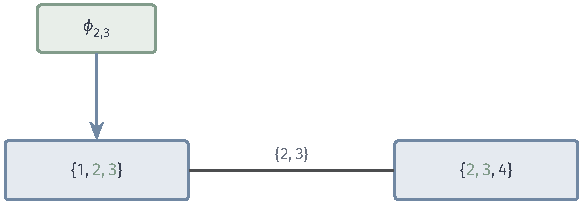
\includegraphics[width=98.651mm]{figures/03-graphs/04-local-functions-and-dynamic-programming/tikz/dp-single-factor-owner/figure.pdf}
  \caption{共享变量不意味着重复计入局部项。两个袋均包含$\phi_{2,3}$的作用域，图中选择左袋作为唯一归属。袋树横边仅表示接口连接，向下的蓝色箭头表示局部项归属，二者含义不同。}
  \label{fig:graph-dp-single-factor-owner}
\end{figure}

\paragraph{消元表示中的归属}
用消元森林表示结构时，归属有一条自然的规则：把$\phi_a$归入$S_a$中最早被消去的变量所对应的袋。第~\ref{sec:graph-dp-clusters-to-decomposition}小节已经说明这个袋包含$S_a$。这条规则恰好对应消元的实际过程：$\phi_a$在它的某个变量第一次被消去时被取出。作用域全在保留集$R$内的局部项（包括作用域为空的常数项）在消元中从不被取出，归入根袋；没有保留集时，常数项可归入任一个根袋。

在四环算例的分解$\{1,2,4\}-\{2,3,4\}$中，$\phi_{1,2}$与$\phi_{1,4}$只能归入$\{1,2,4\}$，$\phi_{2,3}$与$\phi_{3,4}$只能归入$\{2,3,4\}$。按次序$(1,2,3,4)$的消元森林来看，$\phi_{3,4}$本应归入$B_3=\{3,4\}$，这个袋并入$\{2,3,4\}$后归属随之并入。

三元作用域例子的分解中，$\phi_A$只能归入$\{1,2,3\}$，$\phi_B$只能归入$\{2,3,4\}$。

\subsection{选根与求值顺序}
\label{sec:graph-dp-root-order}

给已核验的袋树选根$r$，确定每个非根节点$u$的父节点$p(u)$、子节点集合$\operatorname{ch}(u)$、接口$S_u=B_u\cap B_{p(u)}$与内部变量$I_u=B_u\setminus S_u$（第~\ref{sec:graph-dp-interface-internal}小节）。查询任务使用第~\ref{sec:graph-dp-query-structure}小节保证覆盖保留集$R$的根袋。

求值按袋树的一个后序进行：先处理全部子节点，再处理父节点，最后处理根。每个非根节点只用到子节点交来的表，处理完后把一张以$\bm x_{S_u}$为索引的表交给父节点。后序可以由一次深度优先遍历的完成次序得到，它与根、父节点一样只规定处理次序，在运行中不变。需要恢复配置时，再按前序（后序的逆序，父节点总在子节点之前）走一遍。

原始图不连通时，各分量的袋树之间只有空接口的边相连。沿空接口传递的表只有一项，是一个数：最小成本任务中它是那个分量的最小成本，计数和求和任务中它是那个分量的总数或总和。根把收到的这些数与本分量的结果组合起来，组合方式随任务而定，在各任务中分别说明。

\paragraph{表的存储与对齐}
本地成本、消息和回溯表都是以一组变量为索引的稠密表。为每张表固定变量的排列（例如按编号），各取值按字典序存放，即$(x_{j_1},\ldots,x_{j_k})$像多位数一样以最后一个变量为最低位递增。于是一组取值的位置可以按混合进制直接算出，读取一项按常数时间计；本部分例子中的表都按这种次序列出，例如作用域为$\{2,4\}$的表依次对应$(x_2,x_4)=(0,0),(0,1),(1,0),(1,1)$。

计算时要在袋$B_u$的一组取值$\bm x_{B_u}$上读取$\phi_a(\bm x_{S_a})$或子节点的消息，即从$\bm x_{B_u}$中挑出$S_a$或$S_c$的那几个分量，再算它们在小表中的位置。各变量在$B_u$中的位置事先记下，每次读取就只需几次乘加。接口上的“对齐”指的正是这一步：发送方和接收方按同一组接口变量、同一排列存取消息。

\subsection{消元与袋树的求值对应}
\label{sec:graph-dp-elimination-message-correspondence}

第~\ref{sec:graph-dp-function-message-correspondence}小节在结构上对应了消元簇与袋、剩余作用域与接口。现在在数值上验证这一对应。沿袋树计算时，非根节点$u$先把本地成本与子节点的消息相加，得到
\[
g_u(\bm x_{B_u})=\Phi_u(\bm x_{B_u})+\sum_{c\in\operatorname{ch}(u)}m_{c\to u}(\bm x_{S_c}),
\]
再对内部变量取最小，得到发往父节点的消息
\[
m_{u\to p(u)}(\bm x_{S_u})=\min_{\bm x_{I_u}}g_u(\bm x_{B_u}).
\]
第~\ref{sec:graph-dp-min-cost}节逐项解释这两步。

\begin{theorem}[消元中间函数等于袋消息]
\label{thm:graph-dp-elimination-equals-messages}
设$\pi=(v_1,\ldots,v_k)$是$V\setminus R$的消元次序，袋树由算法~\ref{alg:graph-dp-order-to-decomposition}得到并以消元森林的根（有保留集时为$B_R$）为根，局部项按“作用域中最早被消去的变量”归属，作用域含于$R$的项归入根袋。则按次序消元时，第$i$步取出的函数恰为$\{\phi_a:a\in A_{B_i}\}$与$\{\psi_j:B_j\text{的父袋是}B_i\}$，并且$\psi_i=m_{B_i\to p(B_i)}$。
\end{theorem}

\begin{proof}
消元过程中，当前函数集合里的每个函数，作用域只含尚未消去的变量；它在作用域中第一个变量被消去时被取出，此前一直不动。原始局部项$\phi_a$因此在$S_a$中最早被消去的变量那一步被取出，这正是它的归属。中间函数$\psi_j$的作用域是$S_j$，它在$S_j$中最早被消去的变量那一步被取出，这正是$B_j$的父袋；若$S_j\subseteq R$，它从不被取出，最后留在根袋。这就证明了第一个断言。

再对$i$归纳证明$\psi_i=m_{B_i\to p(B_i)}$。第$i$步取出的函数之和为$\Phi_{B_i}$加上各子袋的$\psi_j$；由归纳假设，后者等于子袋发来的消息，所以这个和就是$g_{B_i}$。$B_i$的内部变量只有$v_i$（第~\ref{sec:graph-dp-function-message-correspondence}小节），所以式~\eqref{eq:graph-dp-elimination-step}的$\psi_i=\min_{x_{v_i}}g_{B_i}$正是消息$m_{B_i\to p(B_i)}$。
\end{proof}

证明只用到“先把取出的函数组合起来，再对一个变量汇总”这一结构，没有用到取最小或相加的具体性质；把它们换成求和与相乘，同样的对应在第~\ref{sec:graph-dp-semiring}节的计数和求和中成立。

\paragraph{合并袋与一次处理多个内部变量}
实际使用的袋树常常把消元森林中相邻的袋合并，例如四环算例把$\{2,3,4\},\{3,4\},\{4\}$并成一个根袋。合并后的袋一次处理多个内部变量：沿袋树的消息是对这些变量同时取最小，而按次序消元则是逐个取最小。由式~\eqref{eq:graph-dp-min-rules}的第一条，对几个变量同时取最小等于逐个取最小，所以合并改变的只是中间表，不改变发往父袋的消息和最终结果。更一般的情形，即任意合法分解、任意满足容纳条件的归属，由第~\ref{sec:graph-dp-min-cost-correctness}小节的不变量统一证明。

\paragraph{例子}
三元作用域例子按次序$(1,4,2,3)$消元，得到的袋树是$\{1,2,3\}\to\{2,3\}\leftarrow\{2,3,4\}$、$\{2,3\}\to\{3\}$，以$\{3\}$为根。各条消息恰好是第~\ref{sec:graph-dp-min-cost-recovery}小节表~\ref{tab:graph-dp-elimination-trace}中的$\psi_1,\psi_4$与消去$x_2$得到的新函数。

第~\ref{sec:graph-dp-tree-messages}小节的树上递推也是这样的特例：对依赖树选定根，以$\{u,p(u)\}$为袋（第~\ref{sec:graph-tree-decomposition}小节宽度为$1$的分解），把$\phi_u$和$\phi_{u,p(u)}$归入这个袋（根的一元项归入任一个含根的袋），接口就是单个变量$p(u)$，袋消息退化为顶点之间的消息。
